\section{Evaluation of Multimedia Frameworks and Codecs}
\label{sec:4}

\subsection{Latency, Quality, and Resolution of Multimedia Frameworks and Codecs}

After evaluating the multimedia frameworks and its associated codecs, we arrive at the statistics of each of the video stream, and from these statistics, we analyze and come to a decision of which framework shows the best results. \par

As from the bitrate column in Table \ref{tab:table-stat}, MJPG-Streamer shows to be the best multimedia framework in our project. The number of processed bits within seconds determines the video quality. The higher the bitrate, the higher is the quality of the streaming video. In our case, MJPG-Streamer shows the best results followed by FFmpeg with the MJPEG codec.

\begin{table}[H]
	\begin{center}
	\caption{Statistics - Input}
	\label{tab:table-stat}
	\begin{tabular}{l | l | l | l | l}
		Frameworks and Codecs & Read at media & Input bitrate &  Demuxed & Stream bitrate \\
		\hline \hline
		cvlc h264 & 8211 KiB & 272 kb\slash s & 6221 KiB & 222 kb\slash s \\
		cvlc mjpeg & 108015 KiB & 3379 kb\slash s & 101973 KiB & 3268 kb\slash s \\
		ffmpeg h264 & 10300 KiB & 901 kb\slash s & 9313 kb\slash s & 830 kb\slash s \\
		ffmpeg mjpeg & 16544 KiB & 1283 kb\slash s & 16495 KiB & 1345 kb\slash s \\
		mjpgstreamer & 80031 KiB & 7301 kb\slash s & 79814 KiB & 7575 kb\slash s   
	\end{tabular}
	\end{center}
\end{table}

The video streams are formed by a sequence of frames which are calculated per given time unit. The higher the frame rate, the smoother the video will be. Table \ref{tab:videoframe} shows the video frame rate, each video streaming framework displays per given time, and the number of lost frames. From the statistics, we can say that there is a higher number of lost frames in CVLC, which can be due to network and bitrate fluctuation.

\begin{table}[H]
	\begin{center}
		\caption{Statistics - Video}
		\label{tab:videoframe}
	\begin{tabular}{l | l | l | l}
		Frameworks and Codecs & Decoded blocks & Displayed frames & Lost frames \\
		\hline \hline
		cvlc h264 & 16.487 & 8.243 & 27 \\
		cvlc mjpeg & 32.765 & 18.002 & 97 \\
		ffmpeg h264 & 4.177 & 2.067 & 0 \\
		ffmpeg mjpeg & 4.710 & 2.376 & 0 \\
		mjpgstreamer & 4.314 & 2.162 & 0 
	\end{tabular}
\end{center}
\end{table} 

Among the two video codecs (H.264, MJPEG) we used, H.264 compresses chunks of video frames at once, whereas MJPEG compresses video frames as a sequence of JPEG images. From Table \ref{tab:videocodec}, we can say that H.264 compresses chunks of video frames, whereas MJPEG has no frame rate as it compresses video frames sequentially. Coming to the video resolution MJPG-Streamer shows High-Definition (HD) video because of its high resolution.

\begin{table}[H]
	\begin{center}
		\caption{Codec details}
		\label{tab:videocodec}
	\begin{tabular}{l | l | l }
		Frameworks and Codecs & Video resolution & Frame rate \\
		\hline \hline
		cvlc h264 & 640x354 & 24\\
		cvlc mjpeg & 752x416 & \\
		ffmpeg h264 & 752x416 & 25\\
		ffmpeg mjpeg & 752x416 & \\
		mjpgstreamer & 1280x720 & 
	\end{tabular}
\end{center}
\end{table}

GStreamer can interconnect with other multimedia frameworks using their available libraries such as codecs. In our project, VLC does not support GStreamer and can only view the video stream on the web browser when it is streamed through a Janus (WebRTC server). Janus, on the other hand, supports multimedia frameworks, such as GStreamer, FFmpeg, etc, and video codecs H.264 and Vp8.

\subsubsection{Video Quality and Resolution of Working Video Streams}

The quality was evaluated with subject to each of the frameworks (see Fig. \ref{fig:cvlc1}, \ref{fig:cvlc2}, \ref{fig:ffmpeg1}, \ref{fig:ffmpeg2}, \ref{fig:mjpg}), and latency was measured by making single short movements in front of the camera and finding the difference between real movements and its appearance in the stream. The pictures of the resolution and the quality of the video streams are shown below: \par

%Fig. \ref{fig:ffmpeg2} shows poor quality in the video due to the high latency and loss of frames during transmission even though the network throughput was equal to the sent video frame rate.

\begin{figure}[ht]
\centering \begin{minipage}[b]{0.45\linewidth}
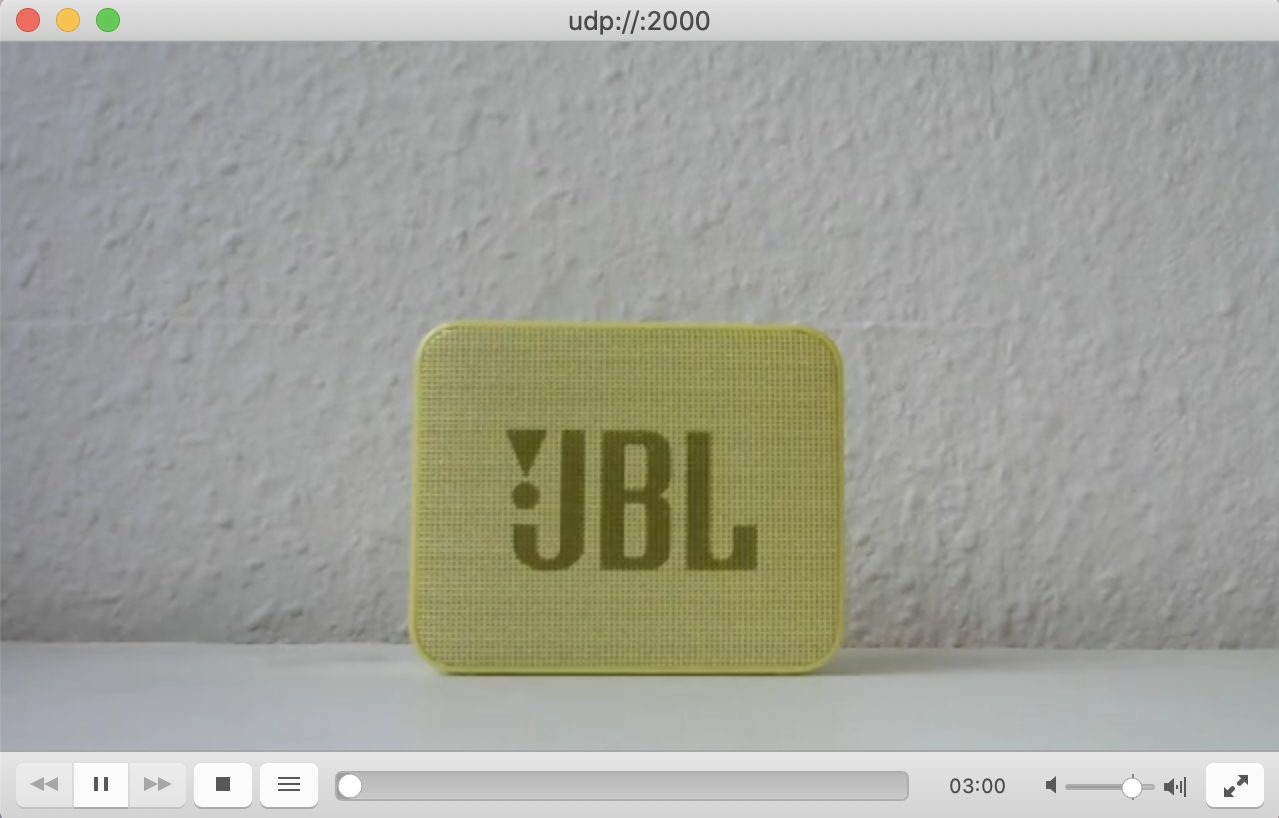
\includegraphics[width=\textwidth]{images/CVLC_H.264.png}
\caption{CVLC H.264} \label{fig:cvlc1}
\end{minipage}
\quad \begin{minipage}[b]{0.45\linewidth}
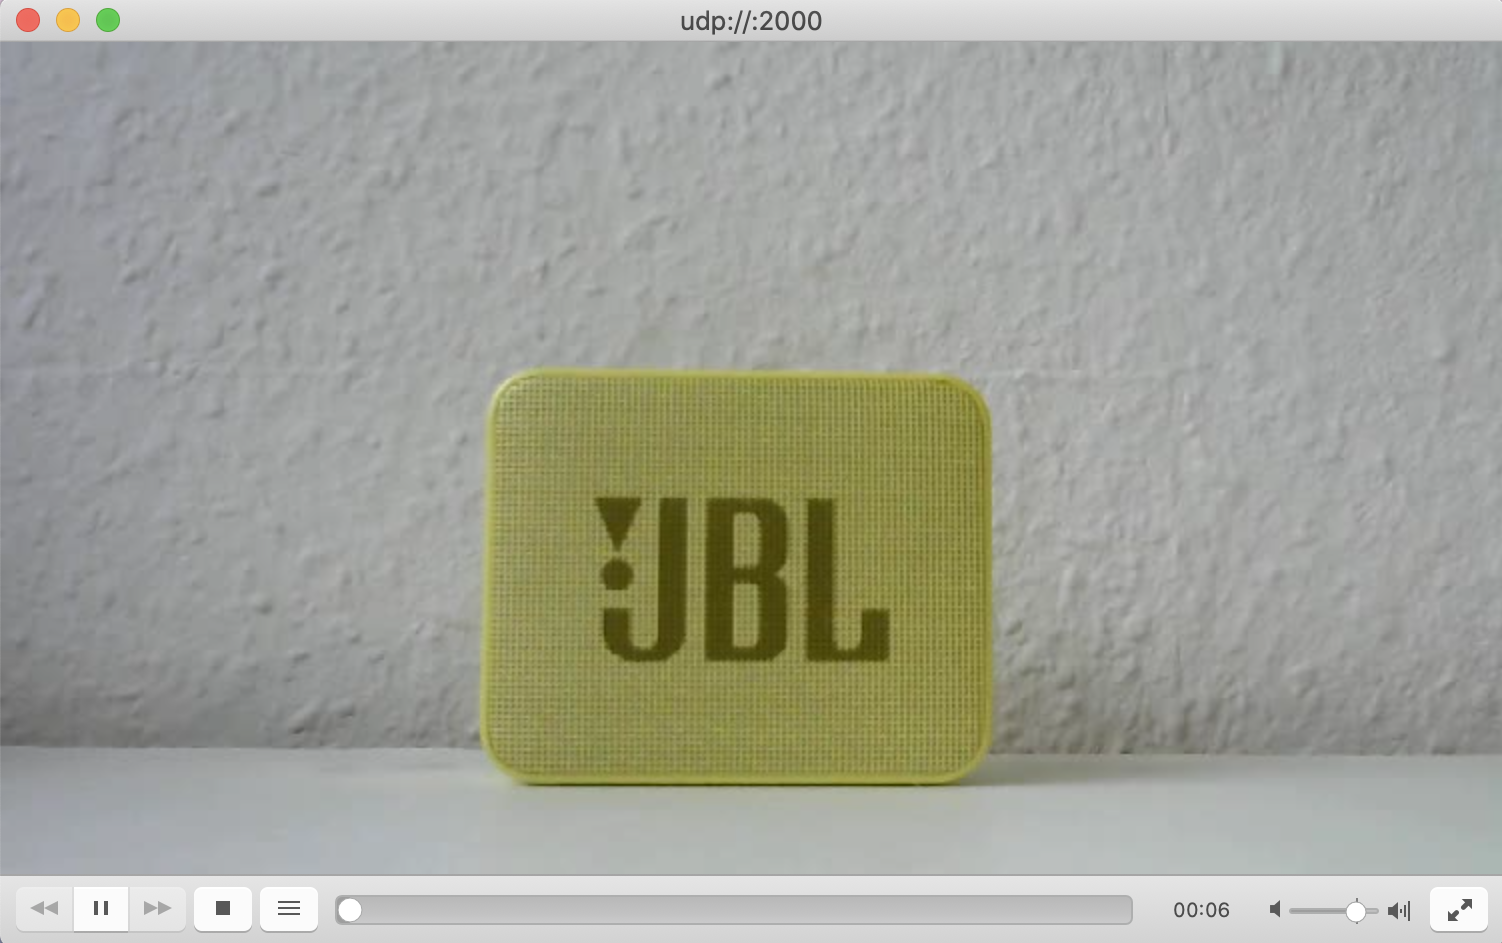
\includegraphics[width=\textwidth]{images/CVLC_MJPEG.png}
\caption{CVLC MJPEG} \label{fig:cvlc2}
\end{minipage}
\end{figure}

\begin{figure}[ht]
\centering \begin{minipage}[b]{0.45\linewidth}
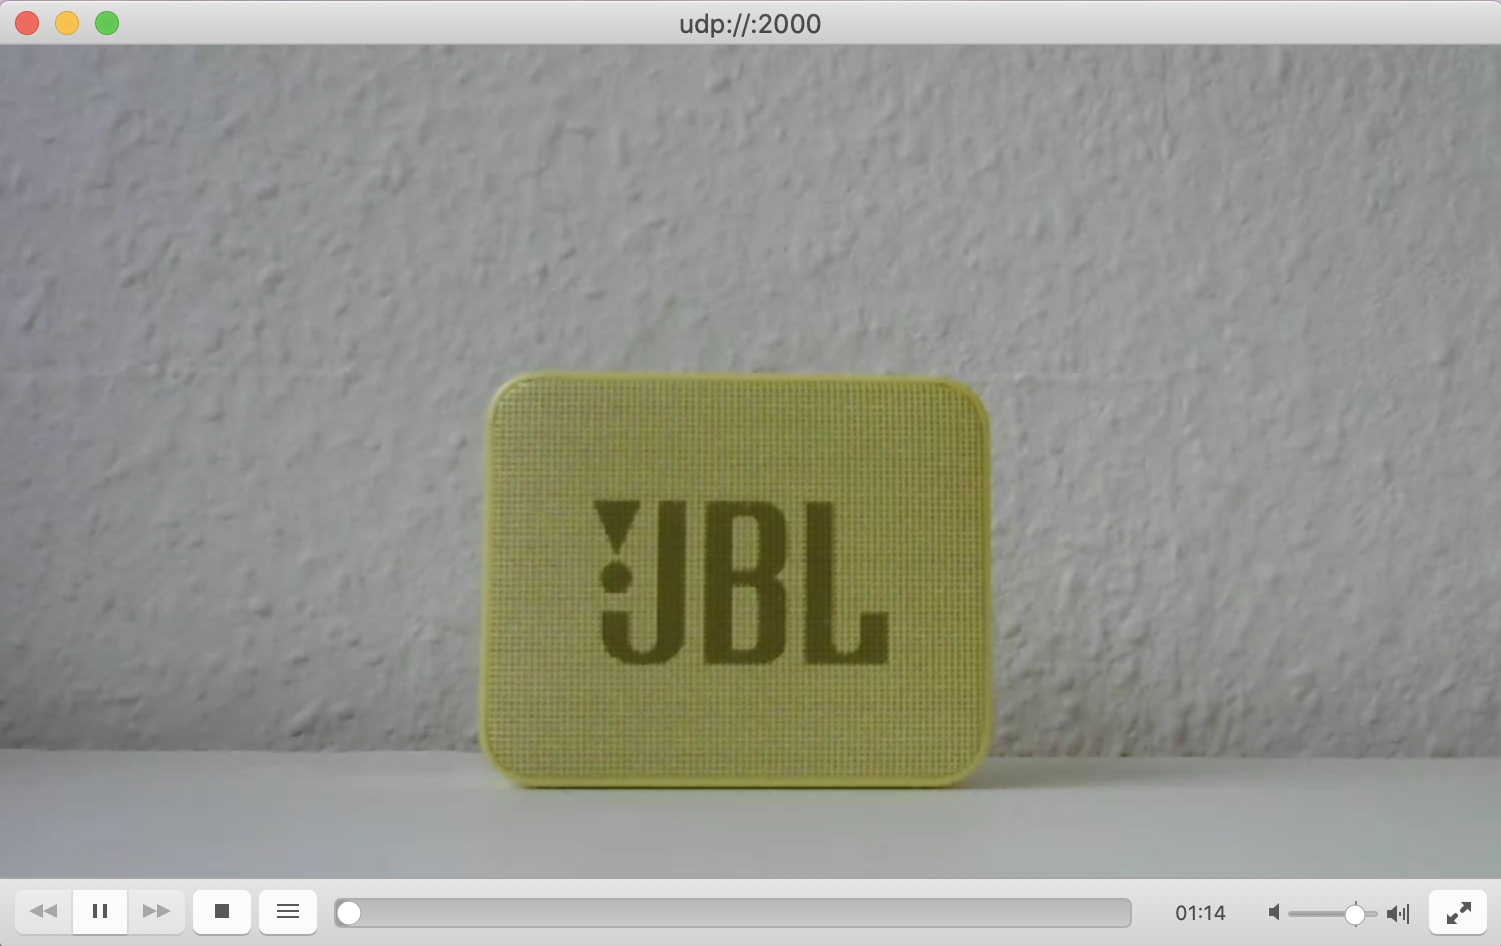
\includegraphics[width=\textwidth]{images/FFmpeg_H.264.png}
\caption{FFmpeg H.264} \label{fig:ffmpeg1}
\end{minipage}
\quad \begin{minipage}[b]{0.45\linewidth}
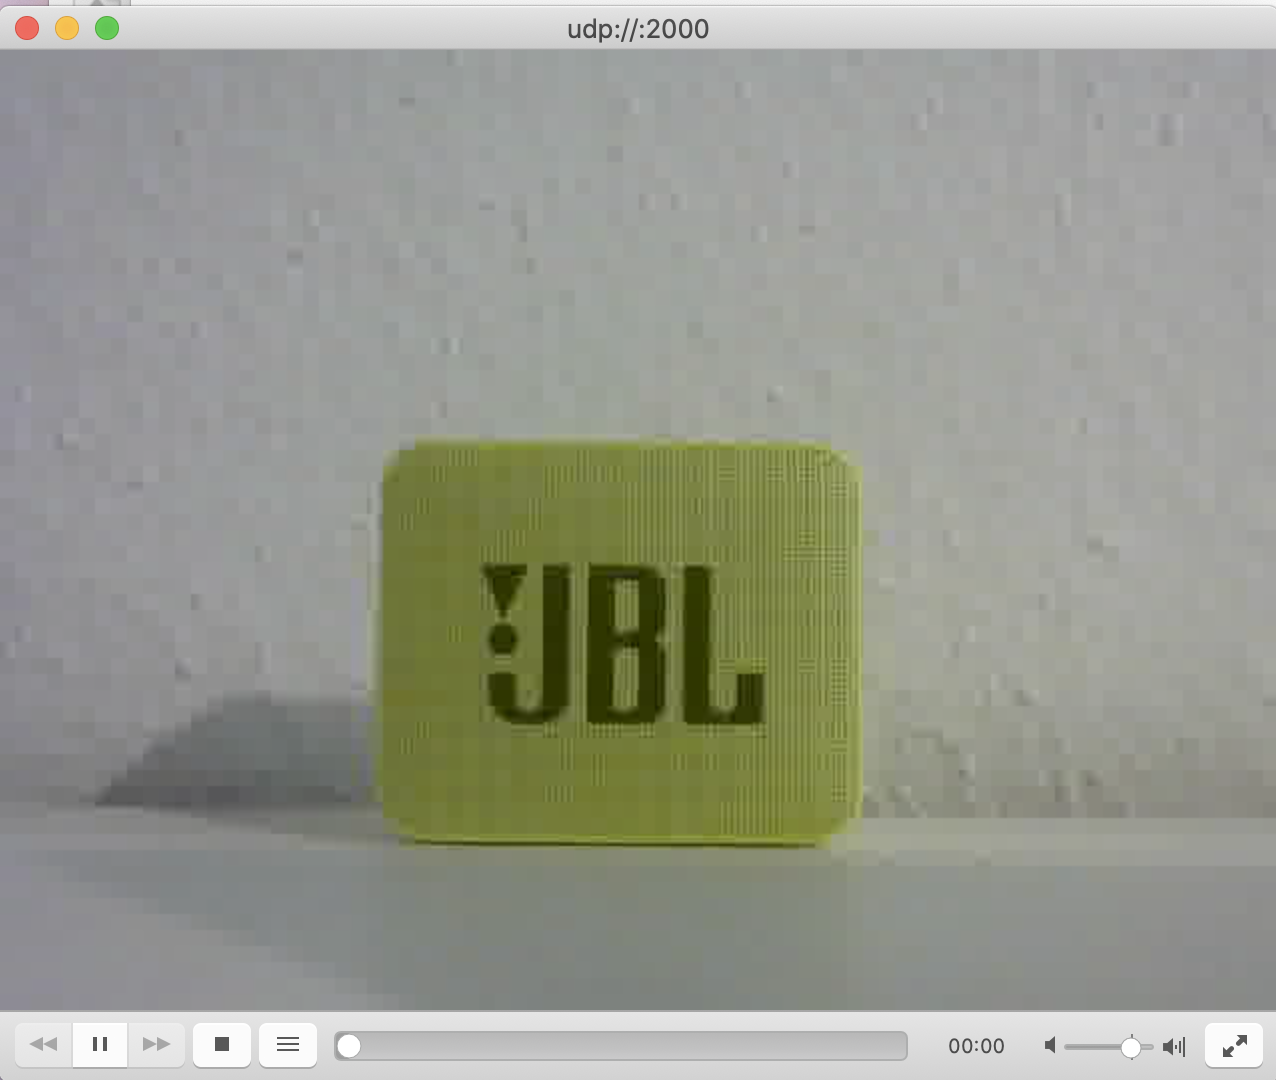
\includegraphics[width=\textwidth]{images/FFmpeg_MJPEG.png}
\caption{FFmpeg MJPEG} \label{fig:ffmpeg2}
\end{minipage}
\end{figure}

\newpage
Fig. \ref{fig:mjpg} of MJPG-Streamer shows a better video quality among all the frameworks because of its high resolution followed by is the FFmpeg with MJPEG (Fig. \ref{fig:ffmpeg2})

\begin{figure}[H]
	\centering
	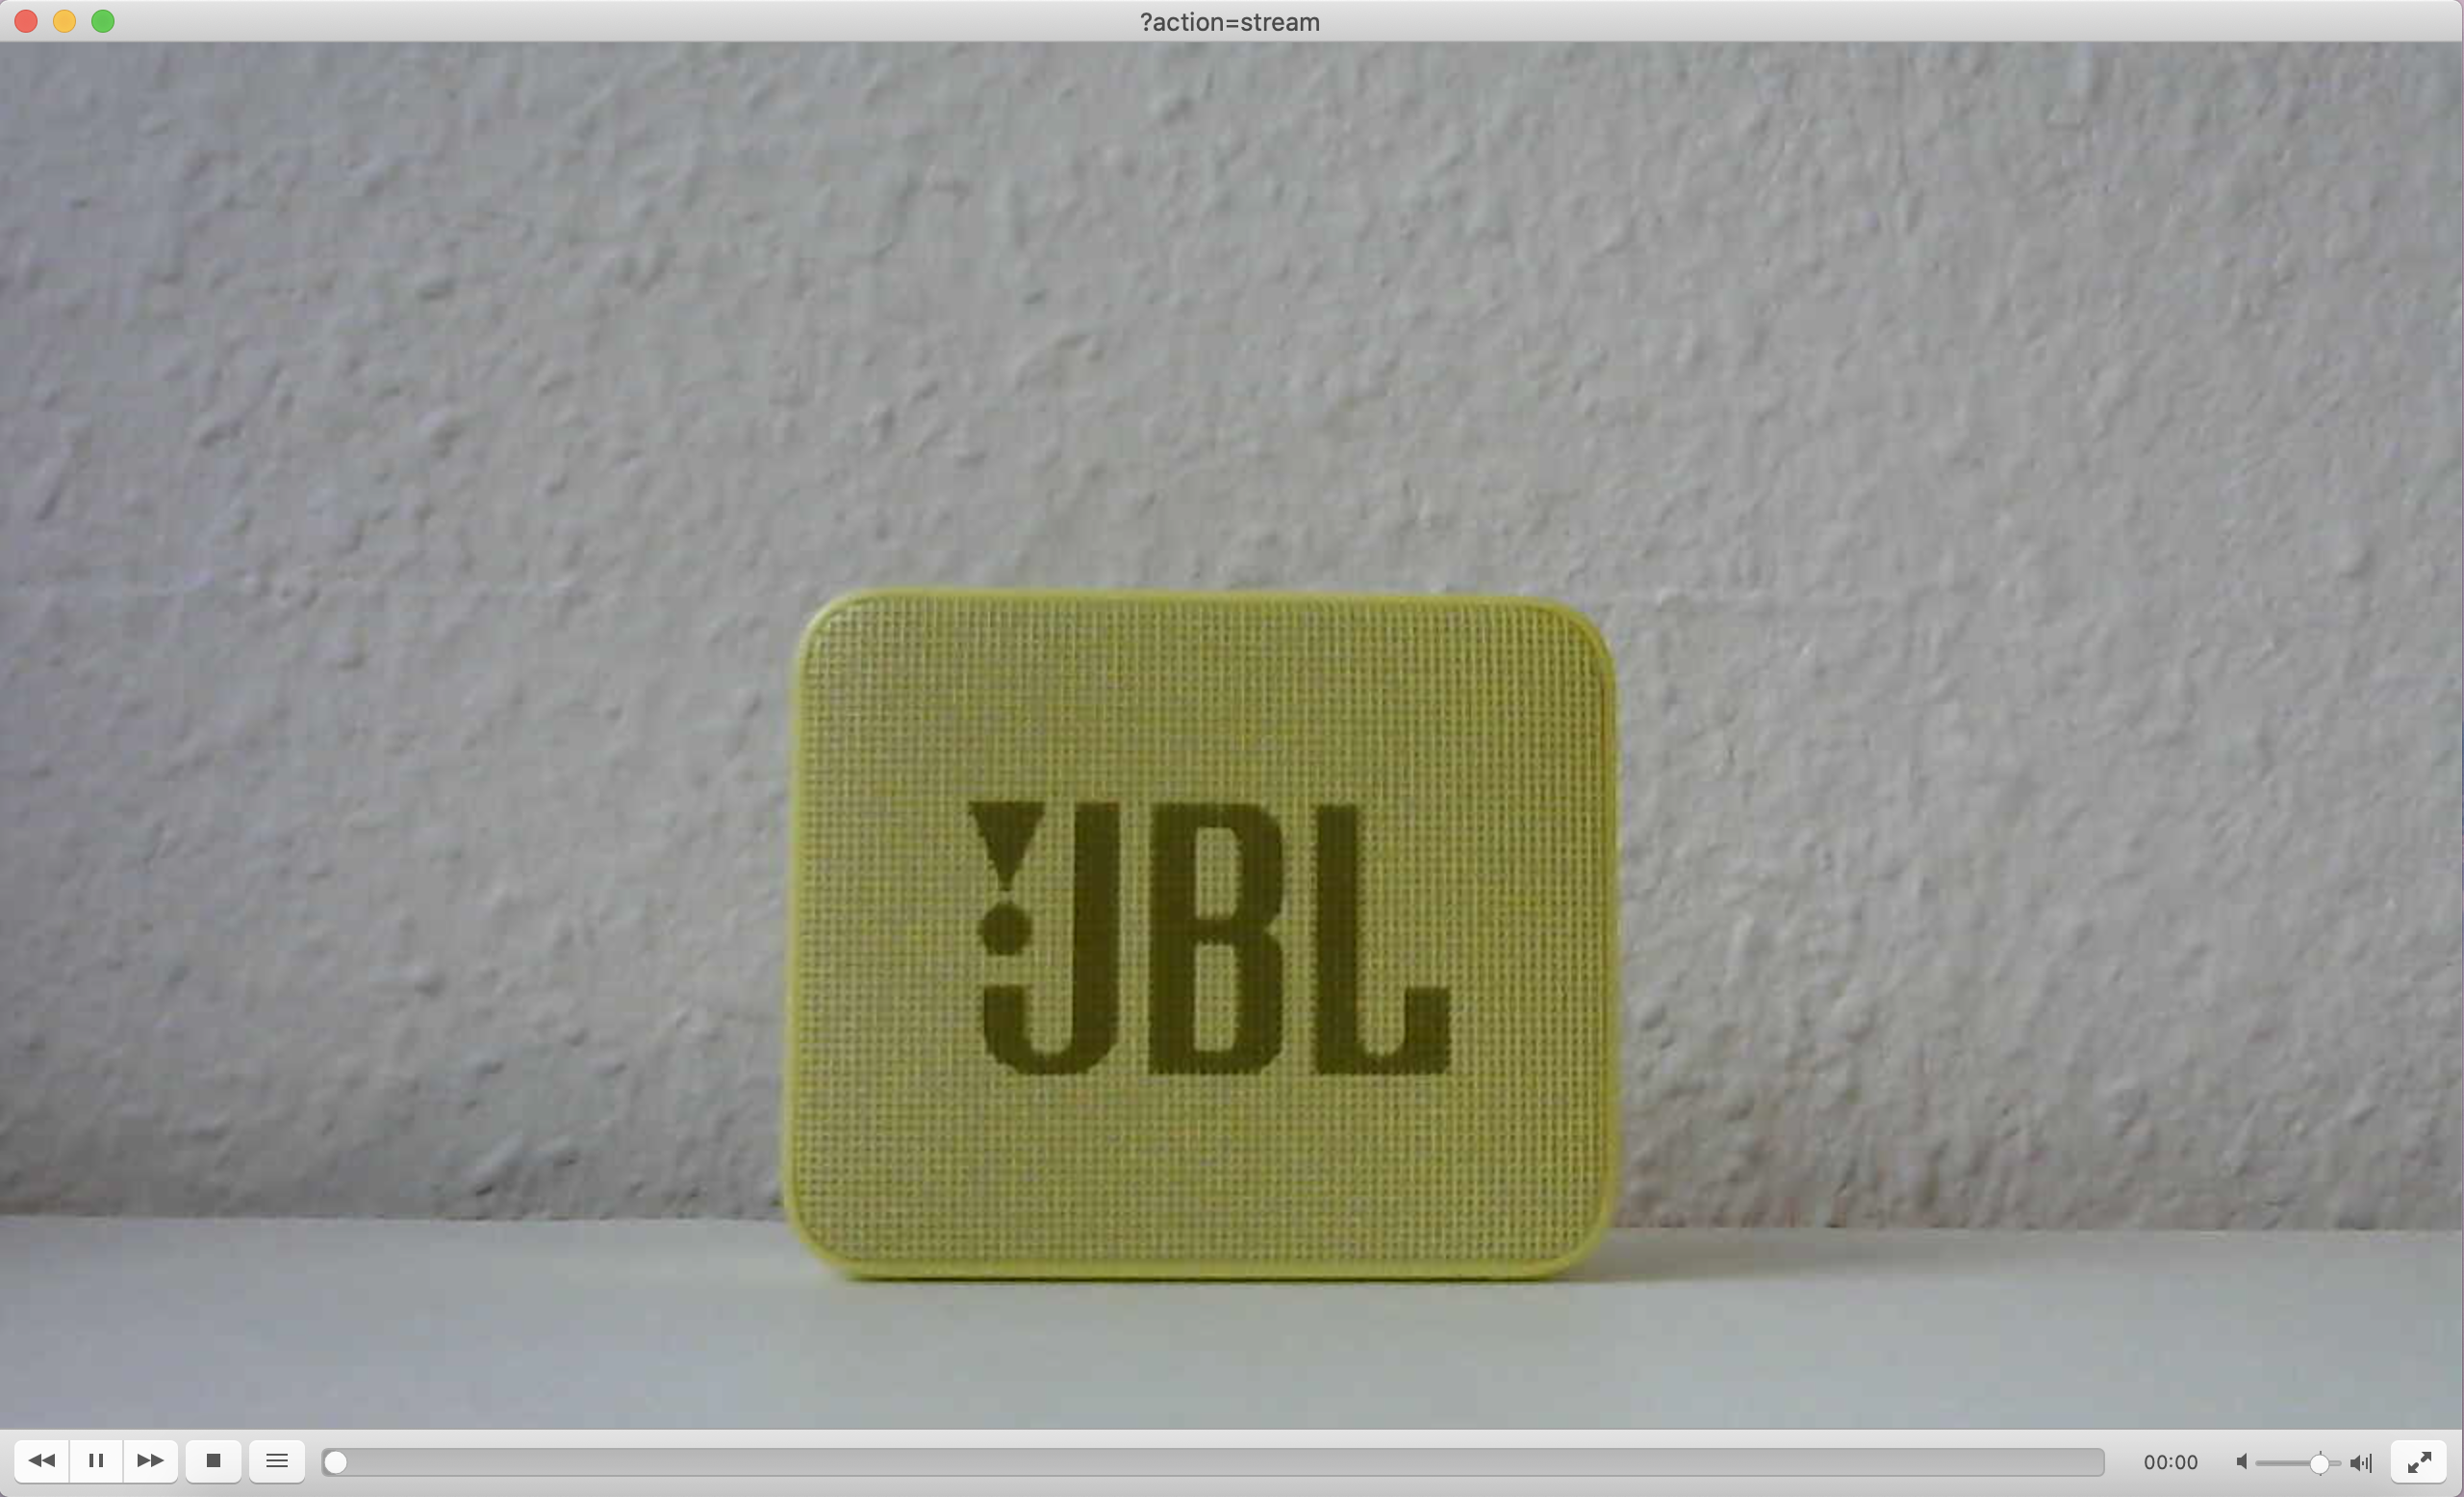
\includegraphics[width=.9\textwidth, trim=4 4 4 4,clip]{images/MJPG-Streamer.png}
	\caption{MJPG-Streamer}
	\label{fig:mjpg}
\end{figure}

At first, we were able to stream video using GStreamer. Subsequently, we couldn’t view the streaming video even though everything is fine from the server-side. We checked the video port from the plug-in configuration file, and we assigned a different port. Still, we couldn’t view the video stream. Fig. \ref{fig:gs} shows the continuous buffering effect. 

\begin{figure}[H]
	\centering
	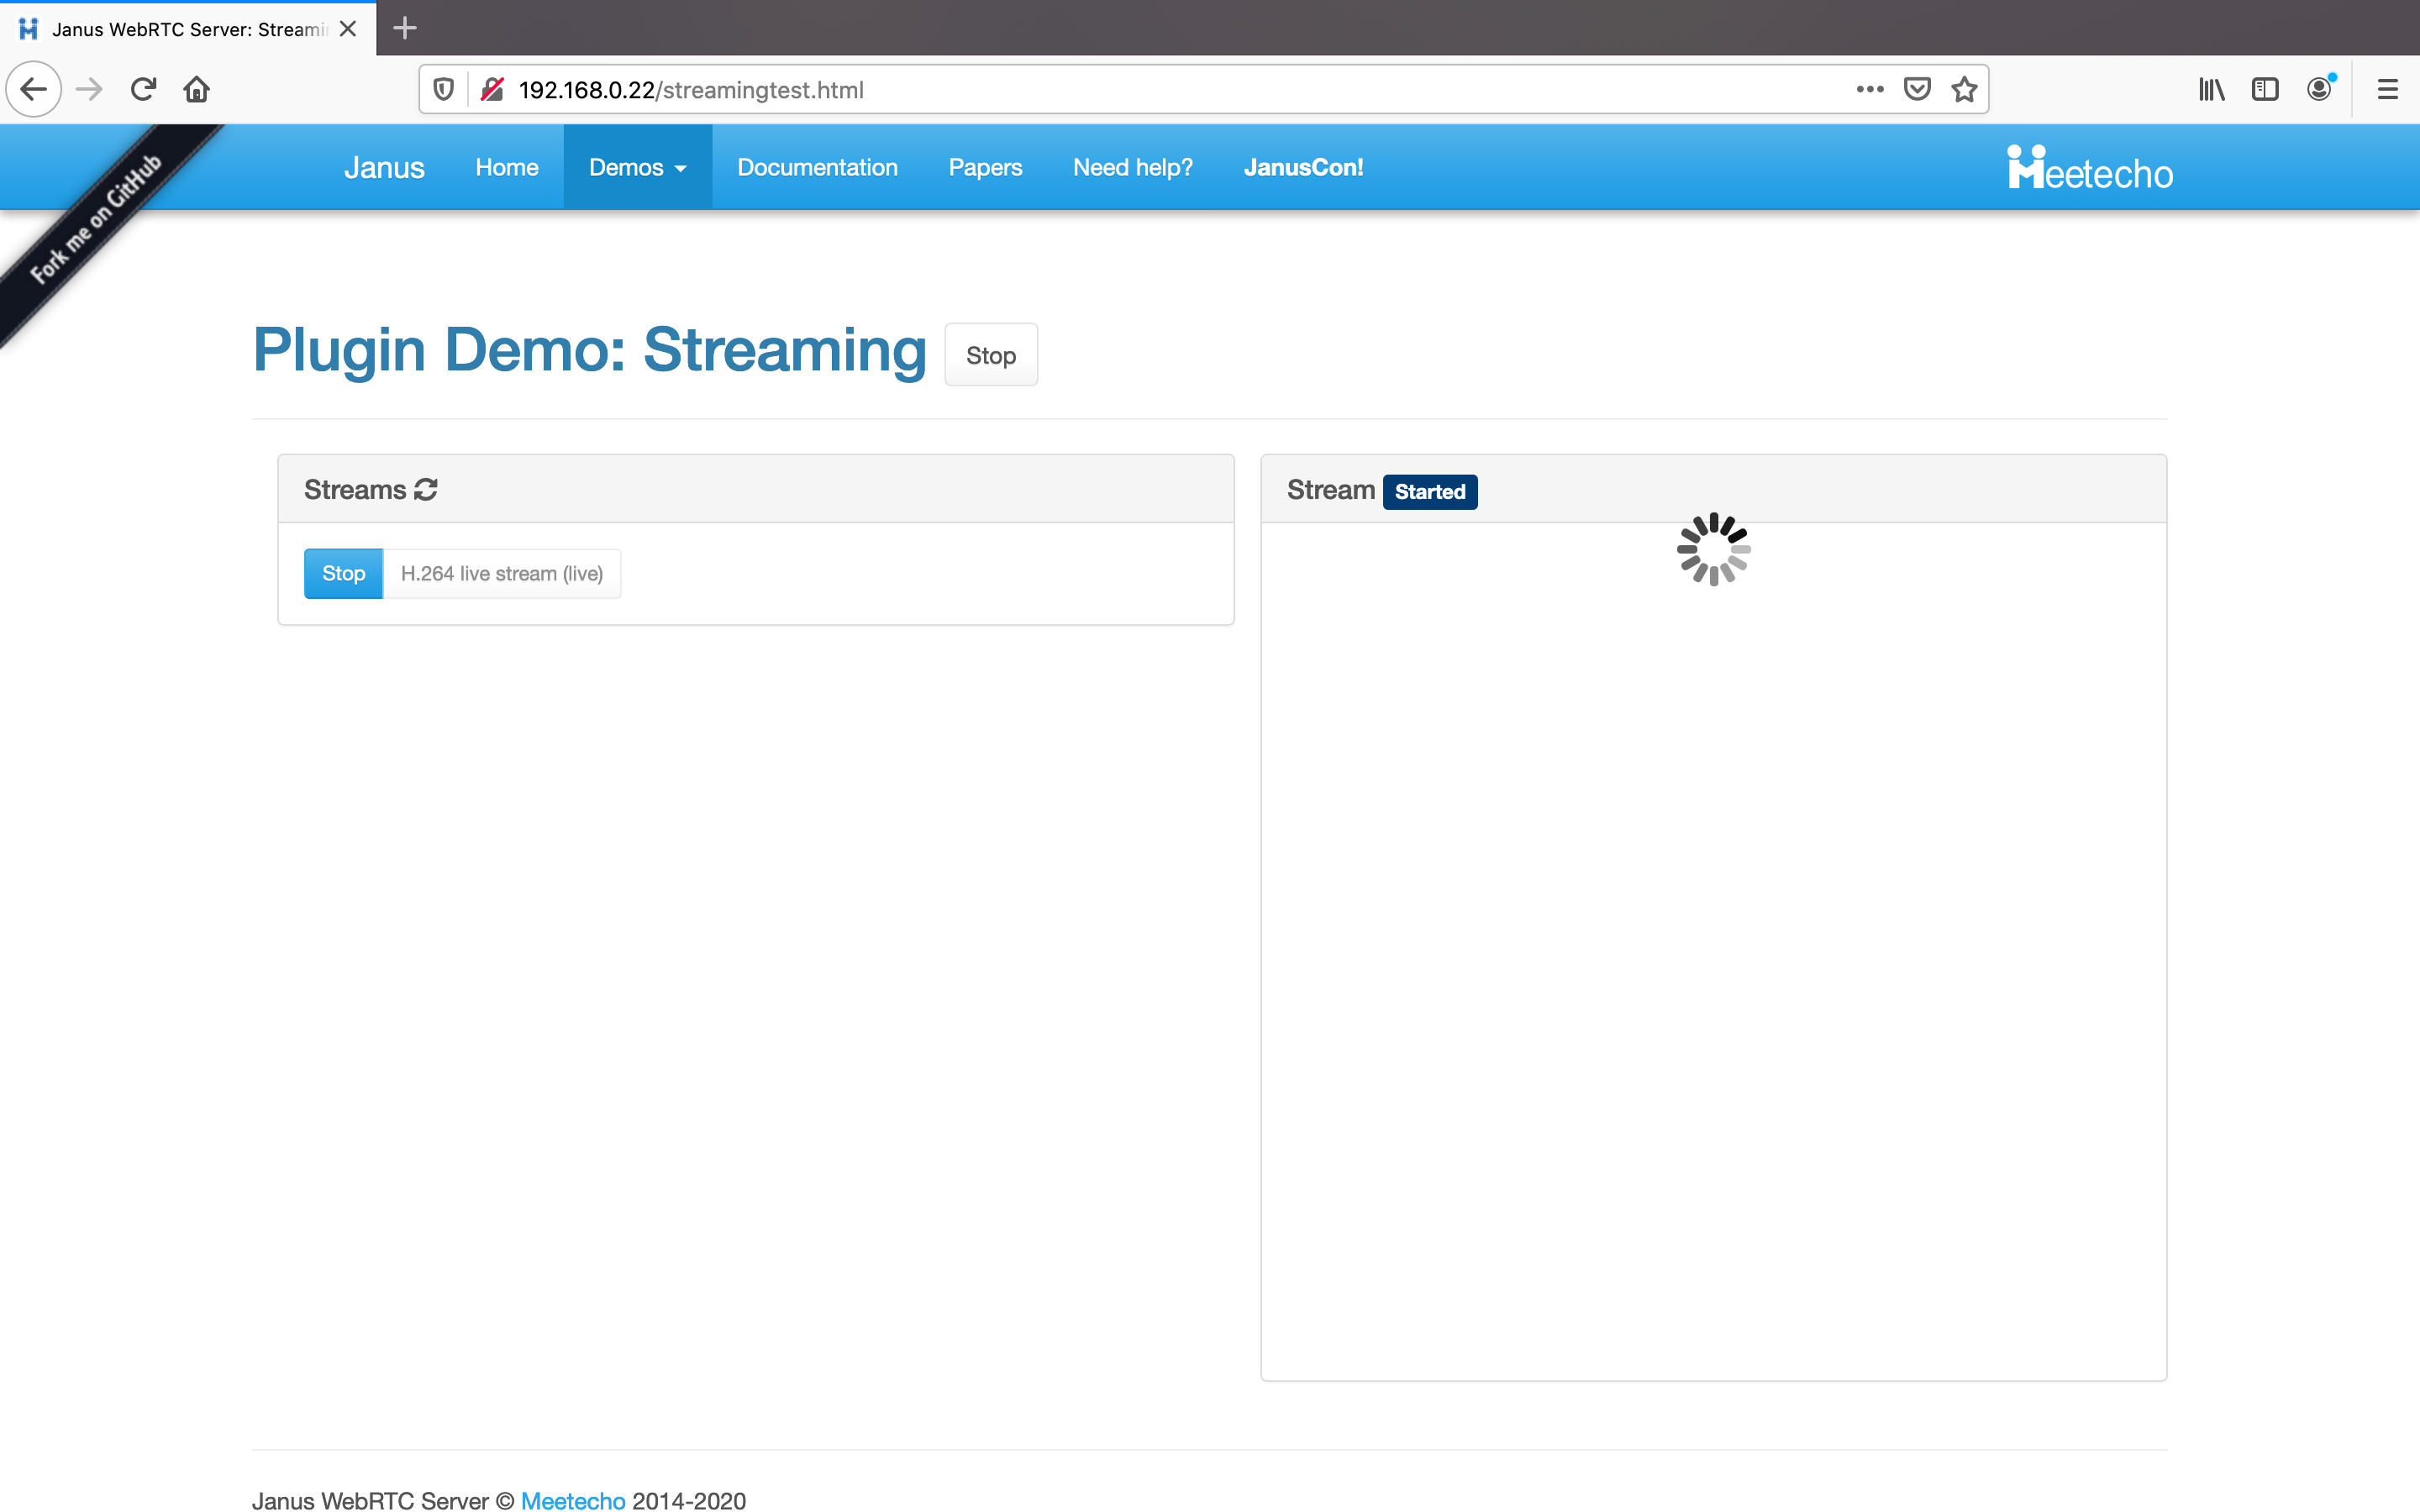
\includegraphics[width=.9\textwidth, trim=4 4 4 4,clip]{images/GStreamer.png}
	\caption{GStreamer H.264}
	\label{fig:gs}
\end{figure}

\subsection{Utilization Comparison of Working Video Streams}

As our main goal in the project is to make a comparison between the multimedia frameworks on RPi3 and RPi4 based on the video quality and resource utilization, we collect the statistics of the multimedia frameworks with its codecs from both RPi3 and RPi4. Based on the statistics, to provide an easy, clear, and descriptive understanding of the data that has been generated, we make use of one of the graphical representations, Boxplot, to provide an illustration of values distributed based on mean, median, and maximum data more precisely in less space. Using Jupyter Notebook we write the Python scripts to draw the boxplots. \par

Here, we make a utilization comparison of RPi3 and RPi4 based on CPU usage, memory usage, and network throughput. \par

For all the multimedia frameworks and codecs, we took seven trials with a time interval of one minute. \par

\textbf{CPU Utilization}:

RPi is a quad-core processor. And when we scrape the metrics for CPU usage of running containers, we get values for all four cores. We calculated the mean for values of four cores to plot the boxplot.

\begin{figure}[H]
	\centering
	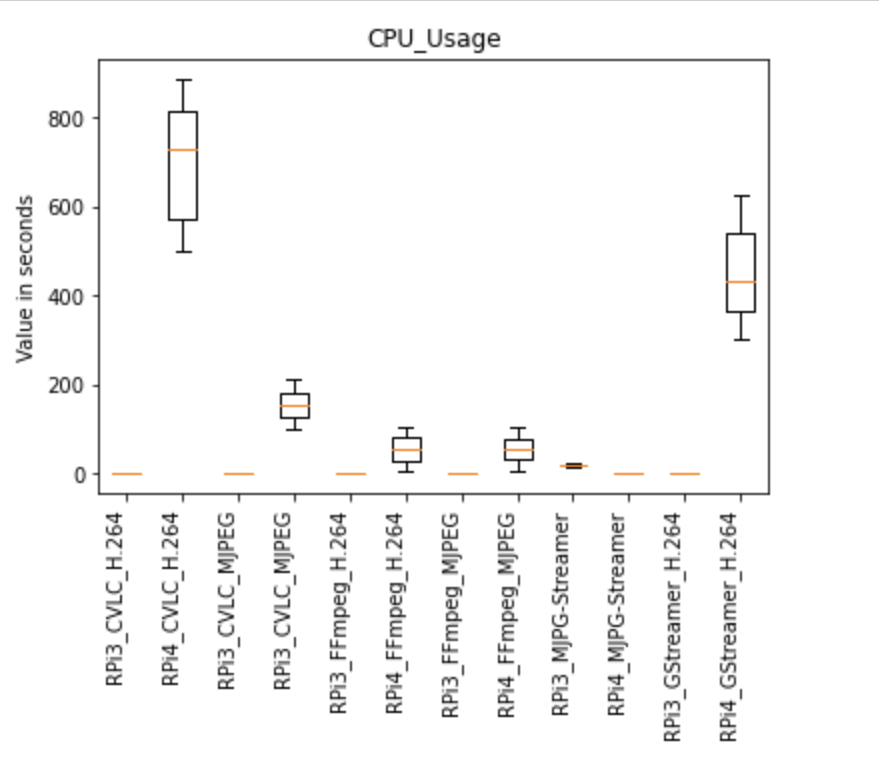
\includegraphics[width=.8\textwidth, trim=4 4 4 4,clip]{images/Boxplots/CPU_Usage.png}
	\caption{CPU Utilization}
	\label{fig:cpu_usage}
\end{figure}

Fig. \ref{fig:cpu_usage} shows the total CPU usage in seconds of all multimedia frameworks with its respective codecs. Unfortunately, in our project, we are unable to view the video stream from the RPi3 except for MJPG-Streamer, which affects the metrics showing no much variation. Hence, we cannot conclude which multimedia framework is best in RPi3. In RPi4, the CPU utilization is high for CVLC (with H.264), which affects the latency, followed by GStreamer (with H.264) because of the running WebRTC container. MJPG-Streamer consumes a minimum amount of CPU followed by FFmpeg (with H.264 and MJPEG), which results in better performance of the system.
  
\textbf{Memory Utilization}:

\begin{figure}[H]
   \centering
   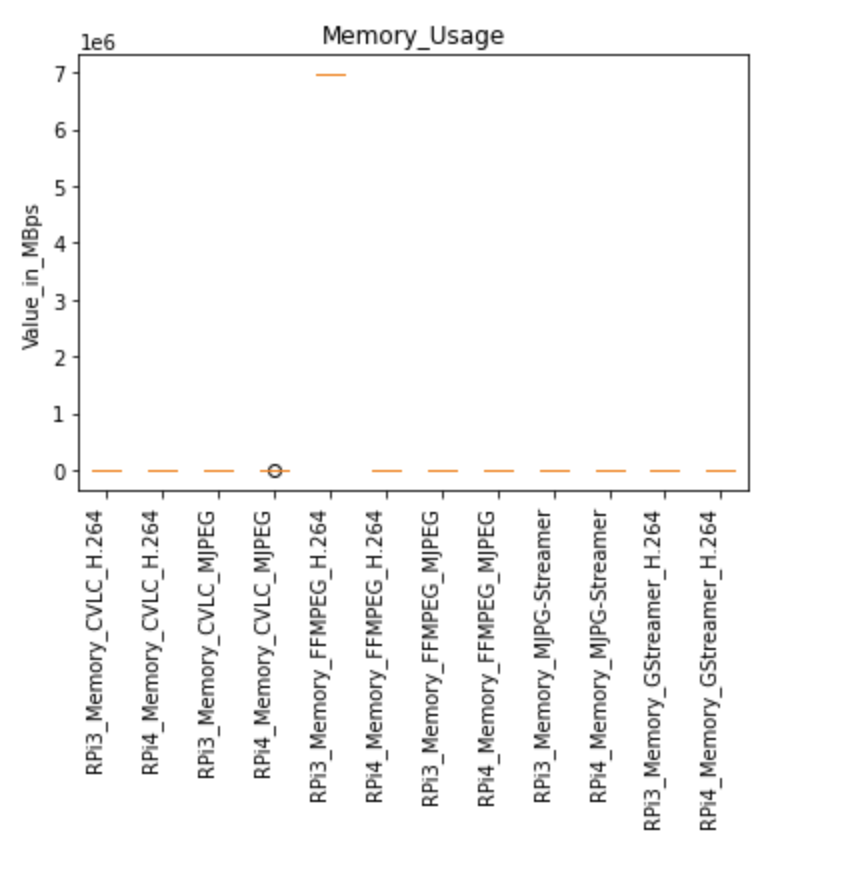
\includegraphics[width=.8\textwidth]{images/Boxplots/Memory_Usage.png}
   \caption{Memory Utilization}
   \label{fig:memory_usage}
\end{figure}

Fig. \ref{fig:memory_usage} shows the total memory usage in Megabytes per second (MBps) of all multimedia frameworks with its respective codecs. Unfortunately, in our project, we are unable to view the video stream from the RPi3 except for MJPG-Streamer, which affects the metrics showing no much variation. Even though there is no video streamed, there is a sudden spike in memory usage for FFmpeg (with H.264), which is uncertain. In RPi4, although all multimedia frameworks have unlimited memory allocation by cAdvisor, they consume a very minimal amount of memory, which is almost fixed across all the frameworks. Hence, we cannot conclude which multimedia framework is best in RPi3 and RPi4 as almost all frameworks consume a minimal amount of memory.

\newpage
\textbf{Network Transmit Total}:

\begin{figure}[H]
   \centering
   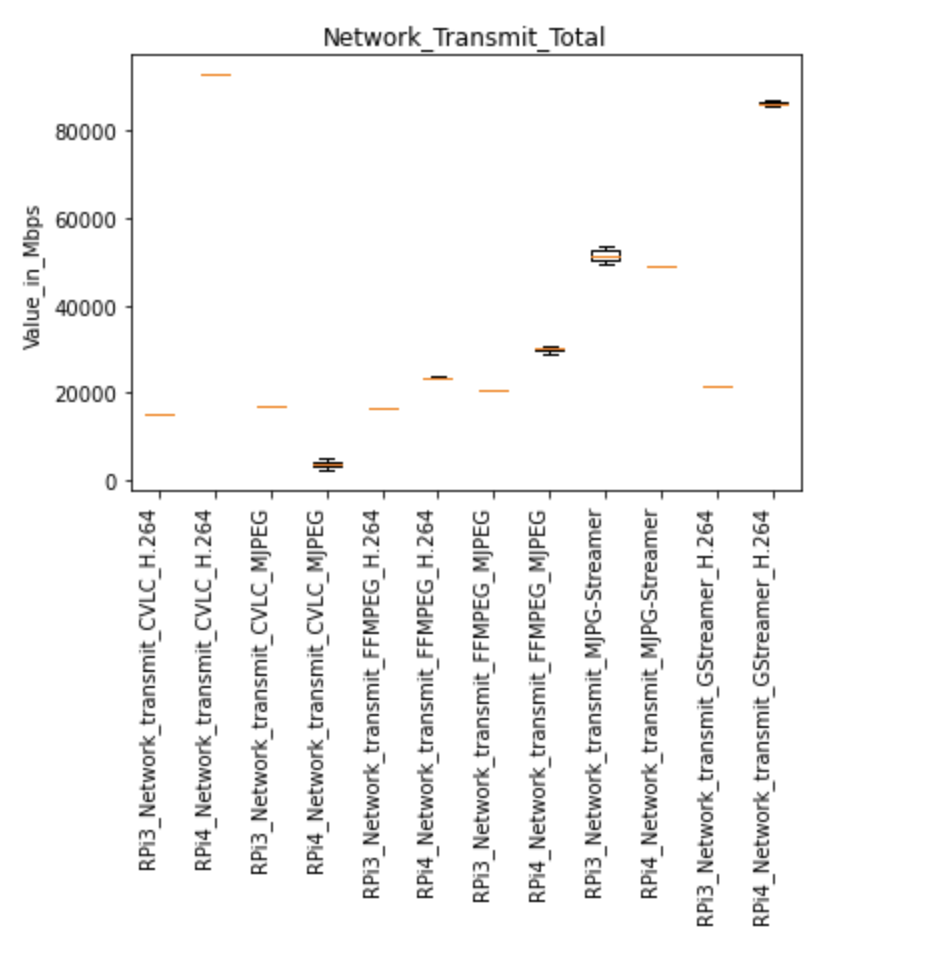
\includegraphics[width=.8\textwidth]{images/Boxplots/Network_Transmit_Total.png}
   \caption{Network Transmit Total}
   \label{fig:network_transmit_total}
\end{figure}

Fig. \ref{fig:network_transmit_total} shows the total network transmission in Megabits per second (Mbps) for all multimedia frameworks with its respective codecs. The higher the bitrate and Network transmission (upstream), the better the video quality, which allows us to send all the allotted video frames over the network. Although we are unable to view the video stream from the RPi3 except for MJPG-Streamer, it shows the variation in values. And from the boxplot, MJPG-Streamer has a higher upstream followed by FFmpeg (with MJPEG), which shows better video quality. In RPi4, GStreamer (with H.264) has a higher upstream because of the running WebRTC container followed by MJPG-Streamer, which shows better video quality.

\newpage
\textbf{Network Receive Total}:

\begin{figure}[H]
   \centering
   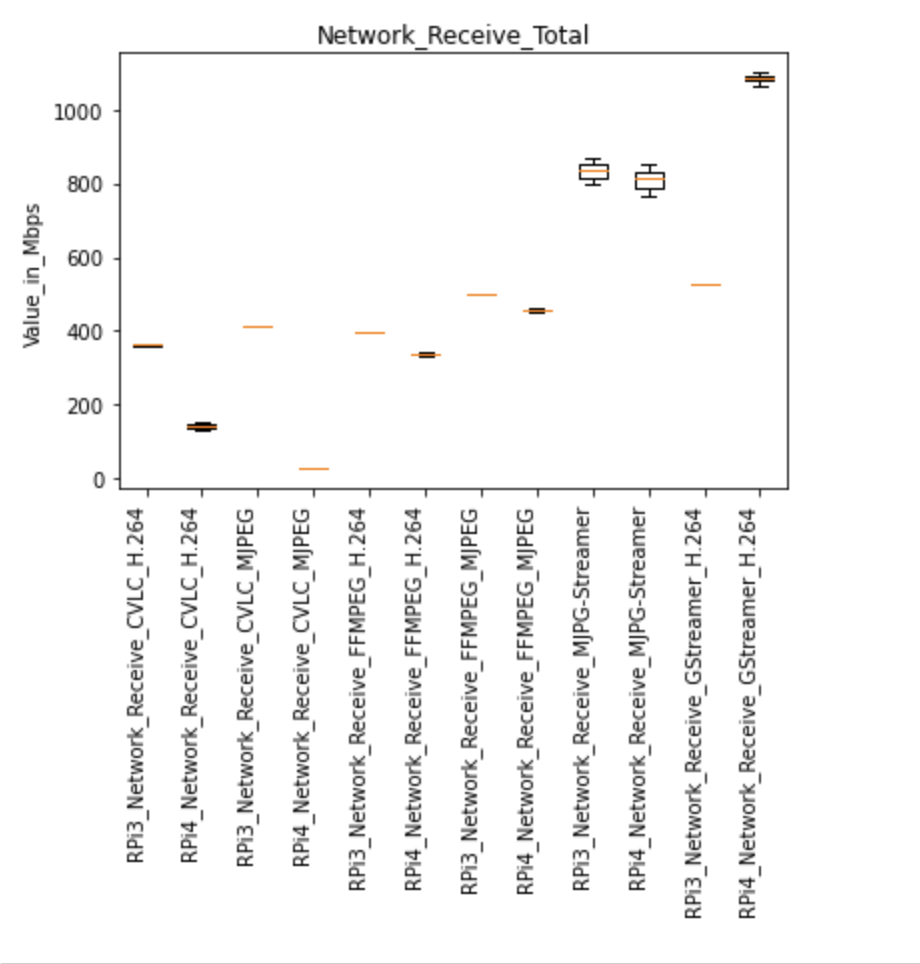
\includegraphics[width=.8\textwidth, trim=4 4 4 4,clip]{images/Boxplots/Network_Receive_Total.png}
   \caption{Network Receive Total}
   \label{fig:network_receive_total}
\end{figure}

Fig. \ref{fig:network_receive_total} shows the total network received in Megabits per second (Mbps) for all multimedia frameworks with its respective codecs. The receiving device receives all the packets sent from the streaming server (RPi).
Although we are unable to view the video stream from the RPi3 except for MJPG-Streamer, it shows the variation in values. And from the boxplot, MJPG-Streamer has higher packets received followed by GStreamer (with H.264), which shows better video quality. In RPi4, GStreamer (with H.264) has higher packets received because of running WebRTC container followed by MJPG-Streamer, which shows better video quality. RPi4 provides better quality of video streaming as its ethernet interface is 100GB, whereas for RPi3 it is 100MB.

The individual boxplots for all the multimedia frameworks and codecs are shown in the Sec. \ref{sec:appendix}.